

\tikzset{every picture/.style={line width=0.75pt}} %set default line width to 0.75pt        

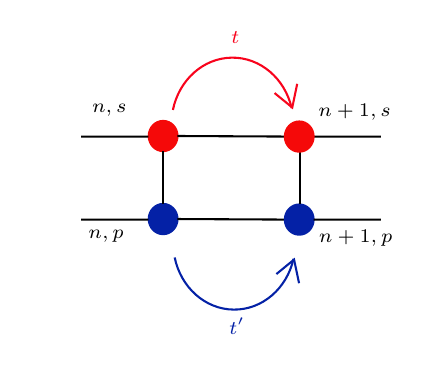
\begin{tikzpicture}[x=0.75pt,y=0.75pt,yscale=-1,xscale=1]
%uncomment if require: \path (0,221); %set diagram left start at 0, and has height of 221

%Shape: Ellipse [id:dp9509974546511886] 
\draw  [color={rgb, 255:red, 245; green, 9; blue, 9 }  ,draw opacity=1 ][fill={rgb, 255:red, 245; green, 9; blue, 9 }  ,fill opacity=1 ] (260.83,66.09) .. controls (260.83,62.08) and (263.93,58.82) .. (267.75,58.82) .. controls (271.58,58.82) and (274.68,62.08) .. (274.68,66.09) .. controls (274.68,70.11) and (271.58,73.37) .. (267.75,73.37) .. controls (263.93,73.37) and (260.83,70.11) .. (260.83,66.09) -- cycle ;
%Straight Lines [id:da6108239084572175] 
\draw    (274.68,66.09) -- (326.4,66.36) ;
%Shape: Ellipse [id:dp6505599276771276] 
\draw  [color={rgb, 255:red, 4; green, 33; blue, 166 }  ,draw opacity=1 ][fill={rgb, 255:red, 4; green, 33; blue, 166 }  ,fill opacity=1 ] (260.83,106.09) .. controls (260.83,102.08) and (263.93,98.82) .. (267.75,98.82) .. controls (271.58,98.82) and (274.68,102.08) .. (274.68,106.09) .. controls (274.68,110.11) and (271.58,113.37) .. (267.75,113.37) .. controls (263.93,113.37) and (260.83,110.11) .. (260.83,106.09) -- cycle ;
%Straight Lines [id:da5080637952717771] 
\draw    (274.68,106.09) -- (326.4,106.36) ;
%Shape: Ellipse [id:dp6408999392104522] 
\draw  [color={rgb, 255:red, 4; green, 33; blue, 166 }  ,draw opacity=1 ][fill={rgb, 255:red, 4; green, 33; blue, 166 }  ,fill opacity=1 ] (326.4,106.36) .. controls (326.4,102.34) and (329.51,99.09) .. (333.33,99.09) .. controls (337.16,99.09) and (340.26,102.34) .. (340.26,106.36) .. controls (340.26,110.38) and (337.16,113.64) .. (333.33,113.64) .. controls (329.51,113.64) and (326.4,110.38) .. (326.4,106.36) -- cycle ;
%Straight Lines [id:da9048962890563637] 
\draw    (340.26,66.36) -- (372.68,66.37) ;
%Straight Lines [id:da8974227202113937] 
\draw    (340.26,106.36) -- (372.68,106.37) ;
%Straight Lines [id:da6458660967437829] 
\draw    (228.26,66.36) -- (260.68,66.37) ;
%Straight Lines [id:da235583538860336] 
\draw    (228.26,106.36) -- (260.68,106.37) ;
%Straight Lines [id:da13127610214656893] 
\draw    (267.75,73.37) -- (267.75,98.82) ;
%Straight Lines [id:da41734146815277795] 
\draw    (333.75,73.37) -- (333.75,98.82) ;
%Shape: Ellipse [id:dp9917459854521972] 
\draw  [color={rgb, 255:red, 245; green, 9; blue, 9 }  ,draw opacity=1 ][fill={rgb, 255:red, 245; green, 9; blue, 9 }  ,fill opacity=1 ] (326.4,66.36) .. controls (326.4,62.34) and (329.51,59.09) .. (333.33,59.09) .. controls (337.16,59.09) and (340.26,62.34) .. (340.26,66.36) .. controls (340.26,70.38) and (337.16,73.64) .. (333.33,73.64) .. controls (329.51,73.64) and (326.4,70.38) .. (326.4,66.36) -- cycle ;
%Shape: Arc [id:dp9460179479043493] 
\draw  [draw opacity=0] (329.7,52.67) .. controls (326.46,38.51) and (314.67,28.12) .. (300.76,28.34) .. controls (286.87,28.56) and (275.36,39.3) .. (272.47,53.53) -- (301.18,60.54) -- cycle ; \draw  [color={rgb, 255:red, 248; green, 3; blue, 28 }  ,draw opacity=1 ] (329.7,52.67) .. controls (326.46,38.51) and (314.67,28.12) .. (300.76,28.34) .. controls (286.87,28.56) and (275.36,39.3) .. (272.47,53.53) ;  
\draw  [color={rgb, 255:red, 247; green, 7; blue, 29 }  ,draw opacity=1 ] (321.45,45.4) -- (329.98,52.36) -- (332.35,40.97) ;
%Shape: Arc [id:dp33186402587230834] 
\draw  [draw opacity=0] (330.57,125.31) .. controls (327.37,139.48) and (315.61,149.91) .. (301.7,149.73) .. controls (287.81,149.56) and (276.26,138.86) .. (273.33,124.63) -- (302.02,117.54) -- cycle ; \draw  [color={rgb, 255:red, 4; green, 33; blue, 166 }  ,draw opacity=1 ] (330.57,125.31) .. controls (327.37,139.48) and (315.61,149.91) .. (301.7,149.73) .. controls (287.81,149.56) and (276.26,138.86) .. (273.33,124.63) ;  
\draw  [color={rgb, 255:red, 4; green, 33; blue, 166 }  ,draw opacity=1 ] (322.33,132.61) -- (330.84,125.62) -- (333.25,137.01) ;

% Text Node
\draw (203,64.4) node [anchor=north west][inner sep=0.75pt]    {$\dotsc $};
% Text Node
\draw (203,103.8) node [anchor=north west][inner sep=0.75pt]    {$\dotsc $};
% Text Node
\draw (376,64.4) node [anchor=north west][inner sep=0.75pt]    {$\dotsc $};
% Text Node
\draw (247,81.4) node [anchor=north west][inner sep=0.75pt]  [font=\scriptsize]  {$\si{\ohm}$};
% Text Node
\draw (340,81.4) node [anchor=north west][inner sep=0.75pt]  [font=\scriptsize]  {$\si{\ohm}$};
% Text Node
\draw (299,14.4) node [anchor=north west][inner sep=0.75pt]  [font=\scriptsize,color={rgb, 255:red, 248; green, 3; blue, 28 }  ,opacity=1 ]  {$t$};
% Text Node
\draw (298,152.4) node [anchor=north west][inner sep=0.75pt]  [font=\scriptsize,color={rgb, 255:red, 4; green, 33; blue, 166 }  ,opacity=1 ]  {$t'$};
% Text Node
\draw (232,49.4) node [anchor=north west][inner sep=0.75pt]  [font=\scriptsize]  {$\ket{n,s}$};
% Text Node
\draw (230.26,109.76) node [anchor=north west][inner sep=0.75pt]  [font=\scriptsize]  {$\ket{n,p}$};
% Text Node
\draw (341.33,109.76) node [anchor=north west][inner sep=0.75pt]  [font=\scriptsize]  {$\ket{n+1,p}$};
% Text Node
\draw (341,49.4) node [anchor=north west][inner sep=0.75pt]  [font=\scriptsize]  {$\ket{n+1,s}$};
% Text Node
\draw (376,103.8) node [anchor=north west][inner sep=0.75pt]    {$\dotsc $};


\end{tikzpicture}
